\section{实验过程记录}
\subsection{问题1:Main Decoder的实现}
\textbf{问题描述:}Main Decoder 需要根据指令高 6 位 opcode,快速判定指令类型(R-type、lw、sw、beq
、addi、jump等),并正确生成多个控制信号,指导后续数据通路的行为。需要同时输出控制 ALU 的粗略操作类型 aluop,供后级 ALU Decoder 精细译码。

\textbf{解决方案:}采用组合逻辑 case 块,根据不同 opcode 设置一组打包的控制
信号(如 regwrite、memtoreg、memwrite、branch、jump 等),并输出对应的 aluop 类型编码。对于 jump 指
令,由于不涉及 ALU 运算,特殊处理 aluop 赋值为无关。整体保证不同指令类型生成的信号组合正确无冲突。
 \subsection{问题2:ALU Decoder的实现}
\textbf{问题描述:}ALU Decoder 需要根据 aluop(主译码器传入)和指令低 6 位 fu
nct 字段(仅对 R-type有效),确定 ALU 执行
的具体运算类型(如加法、减法、逻辑与、或、比较等),输出准确的 alucontrol 控制信号。

\textbf{解决方案:}采用组合逻辑优先判断 aluop 值:当为 Load/Store 
类型时直接输出加法控制码,当为 Branch 类型时直接输出减法控制码;当为 
R-type 类型时根据 funct 字段进一步精确匹配 ALU 操作(如加、减、与、或、SLT),并输出
对应的 alucontrol 编码。若遇非法或未知 funct,输出默认非法操作码(如 3'bxxx 或其他处理)。
\subsection{问题3:指令间被插入0}
\textbf{问题描述:}指令间被插入0
\begin{figure}[H]
    \centering
    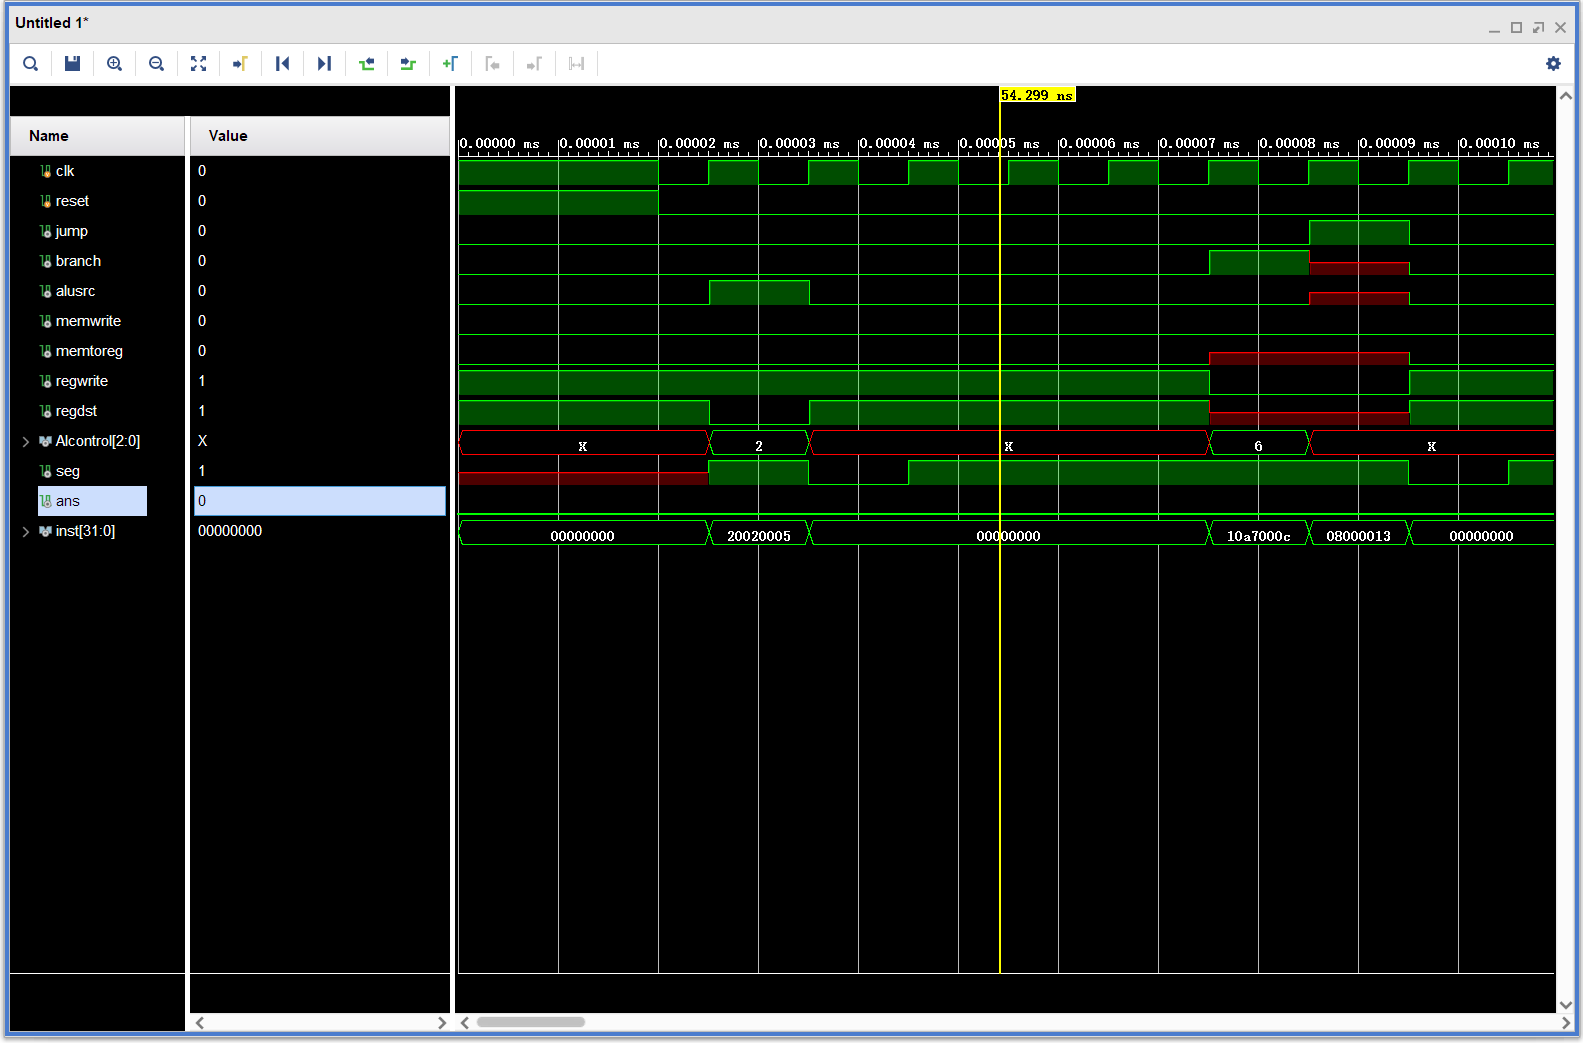
\includegraphics[width=0.9\textwidth]{image/pr.png}
    \caption{指令间被插入0}
    \label{fig:my_label}
\end{figure}
\textbf{解决方案:}重新创建项目,问题解决。